\documentclass[tikz,border=4pt]{standalone}
% Paleta y fuentes compartidas por el libro y las figuras (única fuente de verdad).
\RequirePackage{xcolor}
\definecolor{oxido}{HTML}{B7410E}
\definecolor{cobre}{HTML}{D27D2D}
\definecolor{carbon}{HTML}{2B2B2B}
\definecolor{azul}{HTML}{1F5F8B}
\definecolor{arena}{HTML}{F4EDE4}

\usepackage{fontspec}
\setsansfont{FiraSans}[Extension=.otf,UprightFont=*-Regular,BoldFont=*-SemiBold,ItalicFont=*-Italic,BoldItalicFont=*-SemiBoldItalic]
\setmonofont{FiraMono}[Extension=.otf,UprightFont=*-Regular,BoldFont=*-Medium,Scale=0.95]
\usetikzlibrary{positioning,arrows.meta,calc}
\begin{document}
\sffamily\small
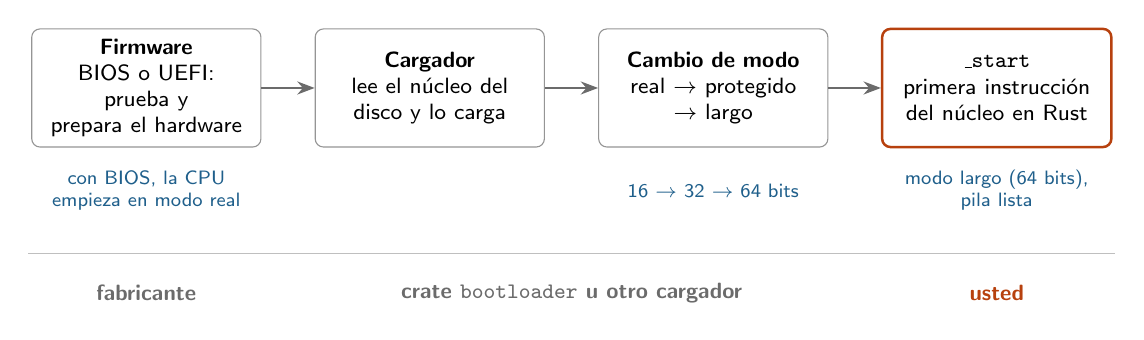
\begin{tikzpicture}[>={Stealth[length=2.2mm]},
  execute at begin node={\hyphenpenalty=10000},
  paso/.style={draw=carbon!50,fill=white,rounded corners=3pt,
    text width=27mm,align=center,minimum height=15mm,
    font=\sffamily\footnotesize,inner sep=3pt},
  modo/.style={font=\sffamily\scriptsize,text=azul,align=center},
  quien/.style={font=\sffamily\footnotesize\bfseries,align=center}]
  \node[paso] (f) at (0,0) {\textbf{Firmware}\\BIOS o UEFI: prueba y\\prepara el hardware};
  \node[paso] (c) at (3.6,0) {\textbf{Cargador}\\lee el núcleo del\\disco y lo carga};
  \node[paso] (m) at (7.2,0) {\textbf{Cambio de modo}\\real $\rightarrow$ protegido\\$\rightarrow$ largo};
  \node[paso,draw=oxido,line width=0.9pt] (s) at (10.8,0) {\textbf{\texttt{\_start}}\\primera instrucción\\del núcleo en Rust};
  \draw[->,thick,carbon!70] (f) -- (c);
  \draw[->,thick,carbon!70] (c) -- (m);
  \draw[->,thick,carbon!70] (m) -- (s);
  \node[modo] at (0,-1.3) {con BIOS, la CPU\\empieza en modo real};
  \node[modo] at (7.2,-1.3) {16 $\rightarrow$ 32 $\rightarrow$ 64 bits};
  \node[modo] at (10.8,-1.3) {modo largo (64 bits),\\pila lista};
  % Quién lo escribe
  \draw[carbon!30] (-1.5,-2.1) -- (12.3,-2.1);
  \node[quien,text=carbon!70] at (0,-2.6) {fabricante};
  \node[quien,text=carbon!70] at (5.4,-2.6) {crate \texttt{bootloader} u otro cargador};
  \node[quien,text=oxido] at (10.8,-2.6) {usted};
\end{tikzpicture}
\end{document}
